% !TEX root = ../thesis.tex
\chapter{Implementierung}\label{ch:implementierung}
In diesem Kapitel wird die Implementierung des Prototyps beschrieben, der das zu realisierende System aus \cref{sec:realisieren} umsetzt.
Dabei werden die wesentlichen Hardwarekomponenten und deren Zusammenspiel erläutert, die für die Umsetzung des Prototyps notwendig sind.
Außerdem wird ein großer Fokus auf die Entwicklung des Definitionsformats für Regeln, Sensoren und externe Datenquellen beschrieben, um die Funktionalitäten des Prototyps zu realisieren.
Anschließend werden die Softwarekomponenten des Systems beschrieben, die für die Umsetzung des Prototyps notwendig sind.
Dazu werden die verwendeten Programmiersprachen und Frameworks für die verschiedenen Softwarekomponenten des Systems erläutert.



\section{Aufbau des Prototyps}
In diesem Abschnitt wird der Aufbau des Prototyps beschrieben, der das zu realisierende System aus \cref{sec:realisieren} umsetzt.
Dabei werden die wesentlichen Hardwarekomponenten und deren Zusammenspiel erläutert, die für die Umsetzung des Prototyps notwendig sind.
Außerdem wird die Verkabelung und Konfiguration der Hardwarekomponenten beschrieben, um den Prototyp betriebsbereit zu machen.

Der Prototyp setzt das zu realisierende System um, das in \cref{sec:realisieren} basierend auf der Konzeption erarbeitet wurde.
Die meisten Komponenten des Systems sind reine Softwarekomponenten, weshalb für diese ein Server benötigt wird, der in einem IP-Netzwerk eingebunden ist.
Die Softwareaspekte dieser Komponenten wird in \cref{sec:programmierung} tiefer behandelt.
Der Sensor- und Aktuatorkoffer selbst ist eine Kombination aus Hardware und Software, wobei die Softwareaspekte in \cref{sec:programmierung} behandelt werden.
Grundlegend benötigt der Prototyp für diese Komponente ein Steuerelement, der die Softwarekomponenten ausführen und die Sensoren steuern kann, eine Stromversorgung und eine Kommunikationsschnittstelle, um mit dem Server zu kommunizieren.
Außerdem werden Sensoren benötigt, die die Umgebung messen und an das Steuerelement weitergeben.

Als Steuerelement kommen verschiedene Geräte infrage, etwa ein Raspberry Pi~\cite{RaspberryPi}, ein Arduino~\cite{Arduino} oder ein ESP32~\cite{ESP32}.
Alle Geräte sind in der Lage, Programme auszuführen und mit Sensoren zu kommunizieren.
Sowohl der Raspberry Pi, als auch der ESP32 verfügen über WLAN-Schnittstellen, wodurch bei diesen Geräten eine kabellose Kommunikation mit dem Server möglich ist, ohne dass zusätzliche Hardware benötigt wird.
Nur der Raspberry Pi verfügt über ein Betriebssystem, wodurch die Softwareentwicklung einfacher ist, da mehr Bibliotheken und Werkzeuge zur Verfügung stehen.
Gleichzeitig ist der Raspberry Pi am teuersten und verbraucht am meisten Strom, weshalb der Arduino und der ESP32 für die entsprechenden Anforderungen besser geeignet sind.
In Abwägung der Vor- und Nachteile wird für den Prototyp ein Raspberry Pi 4\footnote{\href{https://www.raspberrypi.com/products/raspberry-pi-4-model-b/specifications/}{Raspberry Pi 4}} verwendet, da dieser schon vorhanden ist und somit keine zusätzlichen Kosten entstehen, und die Softwareentwicklung einfacher ist.
Auch ein entsprechendes Netzteil ist vorhanden, womit die Stromversorgung gewährleistet ist.
Für einen realweltlichen Einsatz sind andere Faktoren wie Kosten und Energieverbrauch stärker zu berücksichtigen.

Weiterhin sind mehrere Sensoren notwendig, um die Universalität des Systems aufzeigen zu können.
Es existiert eine Vielzahl an Sensoren mit unterschiedlichen Schnittstellen, die für den Prototyp verwendet werden können.
Zu den Schnittstellen gehören unter anderem I2C, SPI, und UART.
Für den Prototyp werden Sensoren mit I2C-Schnittstelle verwendet, da diese Schnittstelle eine einfache Verkabelung ermöglicht und mehrere Sensoren an einem Bus betrieben werden können.
Als Sensoren werden ein Lichtsensor\footnote{\href{https://cdn-shop.adafruit.com/datasheets/TSL25911_Datasheet_EN_v1.pdf}{Lichtsensor TSL2591}} und ein kombinierter Temperatur-, Luftfeuchtigkeits- und Luftdrucksensor\footnote{\href{https://www.bosch-sensortec.com/products/environmental-sensors/humidity-sensors-bme280/}{BME280}} verwendet, welche für viele der Anwendungsfälle geeignet sind.


\begin{figure}[!htb]
	\centering
	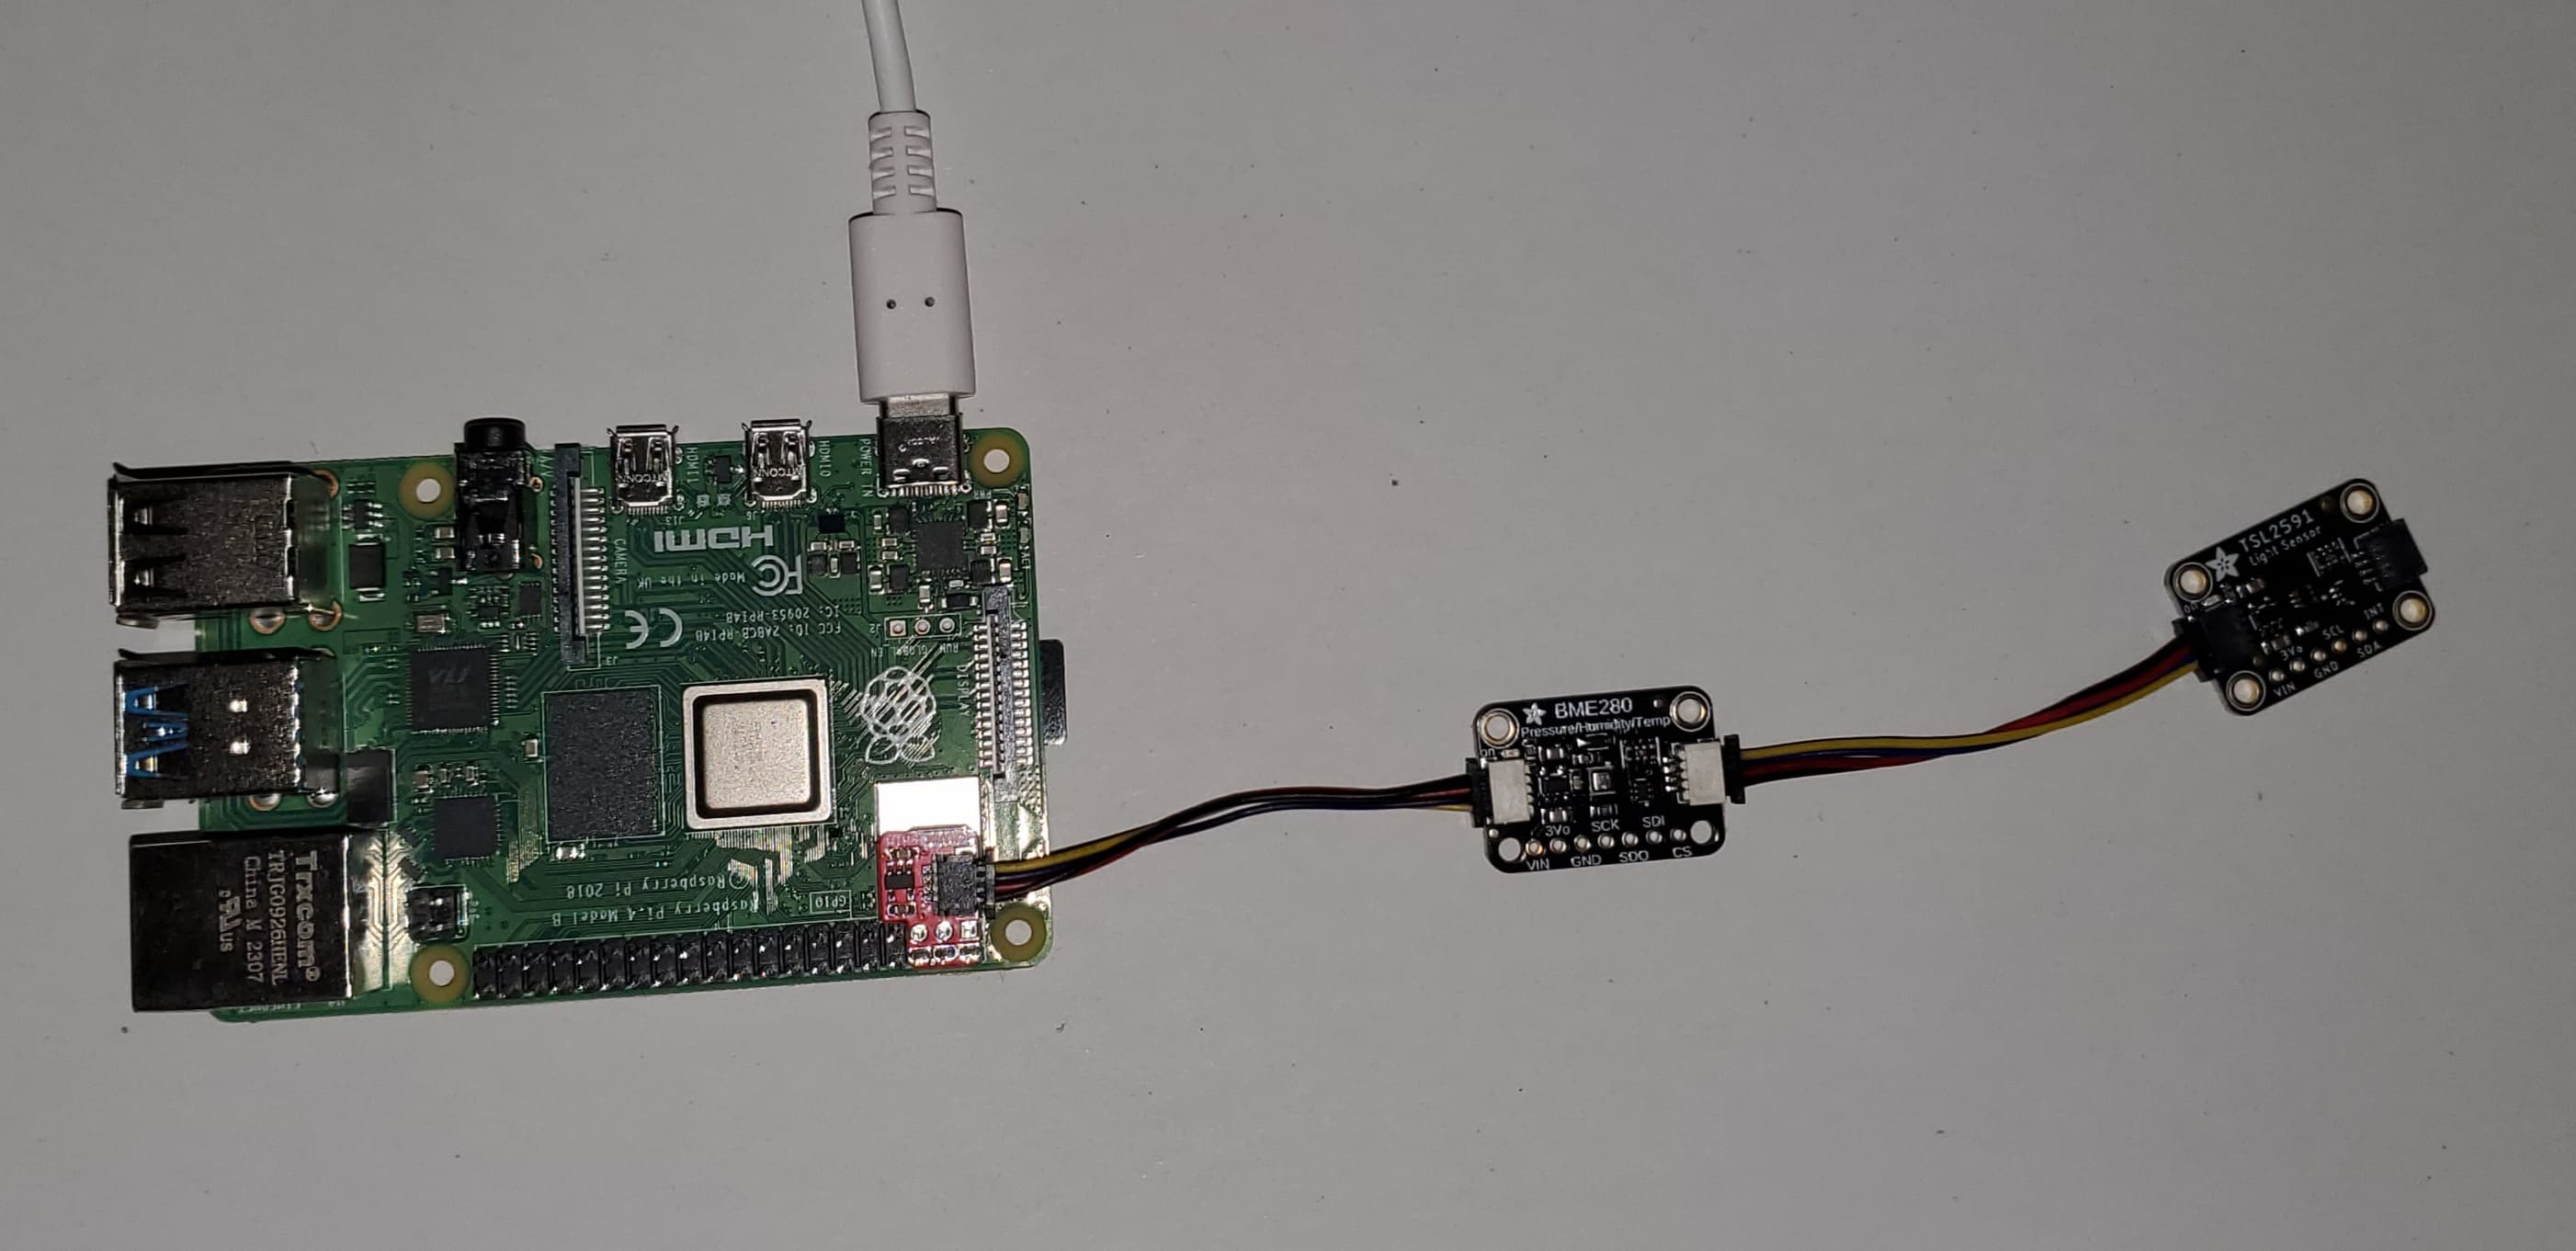
\includegraphics[width=\textwidth]{images/Aufbau.jpg}
	\caption[Aufbau des Prototyps]{Bild des Aufbaus des Prototyps.
		Links ist der Raspberry Pi zu sehen, der als Steuerelement dient.
		Von oben ist der Raspberry Pi mit einem Stromkabel verbunden, das an eine Steckdose angeschlossen ist.
		Rechts sind die beiden Sensoren zu sehen, die hintereinander mit einem Qwiic-Adapter an den Raspberry Pi angeschlossen sind.
	}
	\label{pic:aufbau}
\end{figure}

Der Aufbau des Prototyps ist in \cref{pic:aufbau} dargestellt.
Die Sensoren müssen mit dem Steuerelement verbunden werden, um die Messwerte an das Steuerelement zu übermitteln.
Dafür bieten die Breakout-Boards der Sensoren Qwiic Anschlüsse, die an einen Qwiic-Adapter angeschlossen werden können.
Der Qwiic-Adapter wird an den Raspberry Pi angeschlossen, um die Sensoren mit dem Steuerelement zu verbinden.
So können die Sensoren einfach angeschlossen und betrieben werden, ohne dass eine aufwendige Verkabelung notwendig ist.

Zusammengefasst besteht der Prototyp aus einem Raspberry Pi, der als Steuerelement dient, und zwei Sensoren, die an den Raspberry Pi angeschlossen sind.
Als Kommunikationsschnittstelle wird WLAN verwendet, um mit dem Server zu kommunizieren.
Der erste Sensor ist ein Lichtsensor, der die Lichtintensität misst, und der zweite Sensor ist ein kombinierter Temperatur-, Luftfeuchtigkeits- und Luftdrucksensor, der die Umgebungstemperatur, -luftfeuchtigkeit und -luftdruck misst.
Im nächsten Abschnitt wird die Programmierung des Prototyps beschrieben, um die Funktionalitäten des Prototyps zu realisieren.



\section{Entwicklung des Prototyps}\label{sec:programmierung}
In diesem Abschnitt wird die Entwicklung der Softwarekomponenten des Prototyps beschrieben, die für die Umsetzung des Systems notwendig sind.
Dabei wird das zu realisierende System aus \cref{sec:realisieren} umgesetzt, welches auf der Konzeption basiert.
Zunächst werden die verwendeten Programmiersprachen und Frameworks für die verschiedenen Softwarekomponenten des Systems erläutert.
Anschließend wird die Entwicklung des Definitionsformates für Regeln, Sensoren und externe Datenquellen beschrieben, um die Funktionalitäten des Prototyps zu realisieren.
Daraufhin wird die Entwicklung des Sensor- und Aktuatorkoffers beschrieben, der die zentrale Komponente des Systems darstellt.
Anschließend wird die Entwicklung des Servers beschrieben, der als Bindeglied zwischen dem Sensor- und Aktuatorkoffer und der Nutzerschnittstelle dient.
Zuletzt wird die Entwicklung der Nutzerschnittstelle beschrieben, die für die Darstellung der Sensordaten und die Konfiguration des Systems zuständig ist.


\subsection{Auswahl der Programmiersprachen und Frameworks}
In diesem Abschnitt wird die Auswahl der verwendeten Programmiersprachen und Frameworks für die verschiedenen Softwarekomponenten des Systems erläutert.
Aufgrund der unterschiedlichen Anforderungen und Funktionen des Systems sind die Softwarekomponenten in drei übergreifende Bereiche unterteilt: den Sensor- und Aktuatorkoffer, den Server und die Nutzerschnittstelle.
Diese Trennung ermöglicht es, für jede Komponente die am besten geeigneten Technologien zu verwenden.

Für den Sensor- und Aktuatorkoffer wird die Programmiersprache Python verwendet, da diese eine Vielzahl an Bibliotheken für die Arbeit mit den Schnittstellen des Raspberry Pi zur Interaktion mit den Sensoren bietet.
Weiterhin kann Pythoncode mit leichten Anpassungen zu MicroPython auf Mikrocontrollern wie dem ESP32 oder Arduino portiert werden, was die Flexibilität und Einsatzmöglichkeiten des Systems weiter erhöht.
Weiterhin stellt der Sensor- und Aktuatorkoffer die zentrale Komponente des Systems dar, deren Subkomponenten direkt implementiert werden müssen, sodass die Verwendung eines Frameworks nicht notwendig ist.

Der Server stellt das Bindeglied zwischen dem Sensor- und Aktuatorkoffer und der Nutzerschnittstelle dar und ist für die Speicherung der Sensordaten sowie die Verarbeitung von externen Datenquellen sowie die Verteilung von Benachrichtigungen zuständig.
Der Prototyp setzt für dieses Mitglied auf eine REST-API, die die Kommunikation zwischen den Bereichen sicherstellt.
Dabei wird der Server nur von den anderen Komponenten angesprochen und antwortet auf diese Anfragen, weshalb eine REST-API ausreichend ist.
Für die Implementierung der REST-API wird das Python-Framework Flask\footnote{\href{https://flask.palletsprojects.com/en/latest/}{Flask}} verwendet, da es eine einfache Implementierung der Schnittstelle erlaubt, den Anforderungen des Prototyps entspricht, sowie ein gängiger Standard für solche Anwendungen ist~\cite{FlaskUsage}.

Die Nutzerschnittstelle des Prototyps ist für die Darstellung der Sensordaten und die Konfiguration des Systems zuständig.
Für die Implementierung der Nutzerschnittstelle wird eine Webanwendung verwendet, die im Browser ausgeführt wird.
Diese Webanwendung basiert auf React als Framework, welches die Programmiersprache JavaScript verwendet.
React ist ein gängiges Framework für die Entwicklung von Webanwendungen, das eine Vielzahl von Bibliotheken unterstützt, die für ein Dashboard nützlich sind, wie Graphen zur Darstellung der Sensordaten~\cite{ReactUsage}.

Zusammengefasst wird für den Sensor- und Aktuatorkoffer Python, für den Server Python mit Flask und für die Nutzerschnittstelle JavaScript mit React verwendet.
Im nächsten Abschnitt wird die Entwicklung des Definitionsformates für Regeln, Sensoren und externe Datenquellen beschrieben, um die Funktionalitäten des Prototyps zu realisieren.


\subsection{Entwicklung des Definitionsformats für Regeln, Sensoren und externe Datenquellen}
In diesem Abschnitt wird die Entwicklung eines flexiblen Formats zur Definition von Regeln, Sensoren und externen Datenquellen beschrieben.
Außerdem ist ein Platzhalter für die spätere Integration von Aktuatoren vorgesehen.
Die gewählte Struktur basiert auf JSON, da dieses Format einfach zu lesen und zu erweitern ist.

Für eine einfache und universelle Einsetzbarkeit des gesamten Systems ist es wichtig, dass das System flexibel konfiguriert werden kann und für die Zukunft eine einfache Erweiterung ermöglicht.
Dazu gehört auch, dass die Struktur der Konfiguration logisch und einfach zu verstehen ist, um diesen Zielen nicht im Wege zu stehen.
Das Definitionsformat besteht aus vier Hauptkomponenten: \emph{sensors} (Sensoren), \emph{actors} (Aktuatoren), \emph{external} (externe Datenquellen) und \emph{rules} (Regeln), wobei die Aktuatoren nicht implementiert sind.
Für eine Erweiterung des Systems um Aktuatoren kann das Definitionsformat für die Sensoren als Vorlage dienen.


\begin{figure}[!htb]
\begin{lstlisting}[language=json, caption={[JSON Struktur des Definitionsformates]
	Grundlegende JSON Struktur des Definitionsformates.
	Die Sensoren sind in \cref{lst:sensor-struktur} genauer beschrieben.
	Die Aktuatoren sind nicht implementiert.
	Die externen Datenquellen sind in \cref{lst:external-struktur} genauer beschrieben.
	Die Regeln sind in \cref{lst:rule-struktur} genauer beschrieben.
},
	label={lst:grundlegende-struktur}
]
{
	"sensors": {...},
	"actors": {...},
	"external": {...}
	"rules": {...},
}
\end{lstlisting}
\end{figure}
\begin{figure}[!htb]
\begin{lstlisting}[
	language=json,
	caption={[Struktur der Sensoren im Definitionsformat.]
	Grundlegende Struktur der Sensoren im Definitionsformat.
	Dargestellt sind beispielhaft die zwei Sensoren mit den Schlüsseln \emph{s\_temperature} und \emph{s\_weather}.
	Die Aktionen für einen Sensor des Typs I2C werden in \cref{lst:sensor-aktionen} genauer beschrieben.
	},
	label={lst:sensor-struktur}
]
"sensors": {
	"s_temperature": {
		"name": "Temperature of the shed in degrees Celsius",
		"type": "I2C",
		"i2c_address": "0x77",
		"actions": [...],
		"factor": 0.0095105250,
		"offset": -273.15,
		"msb_first": false
	},
	"s_weather": {
		"name": "Weather",
		"type": "network"
	}
}
\end{lstlisting}
\end{figure}

Jeder Sensor erhält eine eindeutige ID als Schlüssel und kann verschiedenen Typen zugeordnet werden, wie I2C-Sensoren oder Netzwerksensoren.
Diese Struktur ist erweiterbar, sodass in Zukunft weitere Sensortypen hinzugefügt werden können.
Als \emph{type} (Typ) sind für den Prototyp \emph{i2c} (I2C-Sensoren) und \emph{network} (Netzwerksensoren) implementiert, wobei je nach Sensortyp unterschiedliche Informationen benötigt werden.
Für I2C-Sensoren sind etwa die \emph{i2c\_address} (I2C-Adresse), die an den Sensor zu sendenden \emph{actions} (Steuerbefehle), einen \emph{factor} (Korrekturfaktor) einen \emph{offset} (Versatz) für den Messwert, und die Reihenfolge der Datenbytes des Ergebnisses über \emph{msb\_first} erforderlich.
Im Beispiel \cref{lst:sensor-struktur} ist die Definition eines über I2C angeschlossenen Temperatursensors und eines Netzwerksensors dargestellt.
Um den Temperatursensor korrekt anzusteuern, wird seine I2C-Adresse \emph{0x77} benötigt, sowie Steuerbefehle, um ihn zu konfigurieren und Messwerte auszulesen.
Der Temperatursensor gibt die Temperatur in keiner normalen Einheit zurück, diese muss zunächst berechnet werden.
Für eine approximative Berechnung der Temperatur in Grad Celsius wird ein Faktor von \emph{0,0095105250} und ein Versatz von \emph{-273,15} verwendet.
Da der Wert in mehreren Bytes zurückgegeben wird, muss die Reihenfolge der Bytes berücksichtigt werden, was durch \emph{false} für \emph{msb\_first} angegeben wird.
Dabei steht MSB für \emph{Most Significant Byte}, was beschreibt, dass das höchstwertige Byte zuerst übertragen wird.

\begin{figure}[!htb]
\begin{lstlisting}[language=json, caption={[Struktur der Aktionen von Sensoren des Typs I2C im Definitionsformat.]
	Grundlegende Struktur der Aktionen von Sensoren des Typs I2C im Definitionsformat.
	Dargestellt sind beispielhaft die Aktionen für den Sensor \emph{s\_temperature}.
	},
	label={lst:sensor-aktionen}
]
"actions": [
	{
		"type": "write",
		"data": [
			"0xF4",
			"0b00100101"
		],
		"length": 0
	},
	{
		"type": "sleep",
		"data": ["1"],
		"length": 0
	},
	{
		"type": "read",
		"data": [
			"0xFA"
		],
		"length": 2
	}
]
\end{lstlisting}
\end{figure}

Für I2C-Sensoren existieren drei verschiedene Aktionen, die im Beispiel \cref{lst:sensor-aktionen} dargestellt sind.
Hierbei handelt es sich um \emph{write} (Schreibaktionen), \emph{read} (Leseaktionen) und \emph{sleep} (Schlafaktionen).
Aktionen sind in einer Liste aufgelistet, wobei die Aktionen nacheinander ausgeführt werden.

Schreibaktionen haben in den \emph{data} (Daten) die zu sendenden Bytes in hexadezimaler, dezimaler oder binärer Darstellung.
In diesem Beispiel wird der Sensor konfiguriert, indem mit dem ersten Byte das Register des Sensors und mit dem zweiten Byte der Wert für das Register gesetzt wird.
Die \emph{length} (Länge) ist hierbei ungenutzt.

Schlafaktionen haben in den Daten die Zeit in Sekunden, die bis zur nächsten Aktion gewartet werden soll.
Damit kann sichergestellt werden, dass der Sensor genügend Zeit hat, um die Messung durchzuführen.

Leseaktionen senden Daten so wie Schreibaktionen, jedoch wird die \emph{length} (Länge) benötigt, um die Anzahl der Bytes anzugeben, die vom Sensor zurückgegeben werden.
Dieser Sensor ist in der Lage, auch andere Messungen als die Temperatur durchzuführen, die durch unterschiedliche Register definiert sind.
Durch die Leseaktion wird aber nur die Temperatur zurückgegeben, die in zwei Bytes kodiert ist.
Eine Liste von Aktionen endet immer mit genau einer Leseaktion, um die Messwerte des Sensors zu erhalten.

\begin{figure}[!htb]
\begin{lstlisting}[
	language=json,
	caption={[Struktur der externen Datenquellen im Definitionsformat.]
	Grundlegende Struktur der externen Datenquellen im Definitionsformat.
	Dargestellt ist beispielhaft die externe Datenquelle \emph{s\_weather}.
	},
	label={lst:external-struktur}
]
"external": {
	"s_weather": {
		"type": "url",
		"url": "https://api.open-meteo.com/v1/forecast
						?latitude=52.8342444419322
						&longitude=10.704168884802847
						&daily=precipitation_probability_max
						&timezone=Europe%2FBerlin
						&forecast_days=3",
		"keys": ["daily", "precipitation_probability_max"],
		"function": "max",
	}
}
\end{lstlisting}
\end{figure}
	

Auch externe Datenquellen, wie APIs, werden über das Definitionsformat abgebildet.
Jede externe Datenquelle erhält ebenfalls eine eindeutige ID, die mit der ID eines Netzwerksensors übereinstimmt.
Für das Beispiel \cref{lst:external-struktur} wird der Sensor aus \cref{lst:sensor-struktur} verwendet, um die Wetterdaten für den Standort des Sensors zu erhalten.
Für externe Datenquellen sind unterschiedliche \emph{type} (Typen) möglich, wobei für den Prototyp nur \emph{url} umgesetzt ist.
Hierbei handelt es sich bei der angegebenen URL um eine API, die ihre Daten im JSON Format zurückgibt.
Über eine Liste von \emph{keys} (Schlüsseln) kann das zurückgegebene JSON der API durchlaufen werden, um den gewünschten Wert zu erhalten.
Zudem kann eine \emph{function} (Funktion) wie das Maximum einer Liste \emph{max} auf die zurückgegebenen Daten angewendet werden.
In diesem Beispiel gibt die API die Wahrscheinlichkeit für Niederschlag für die nächsten drei Tage zurück, wobei das weiter definiert ist, dass das Maximum dieser Werte als Messwert zurückgegeben wird.
Weitere Typen und Funktionen können in Zukunft hinzugefügt werden, um die Flexibilität des Systems zu erhöhen.

\begin{figure}[!htb]
\begin{lstlisting}[
	language=json,
	caption={[Struktur der Regeln im Definitionsformat.]
	Grundlegende Struktur der Regeln im Definitionsformat.
	Dargestellt ist beispielhaft die Regel \emph{r\_temperature\_low}.
	Die Elemente dieser Beispielregel sind in \cref{lst:rule-notify}, \cref{lst:rule-condition}, \cref{lst:rule-sense} und \cref{lst:rule-send} genauer beschrieben.
	},
	label={lst:rule-struktur}
]
"rules": {
	"r_temperature_low": {
		"name": "Check for low temperature",
		"elements": [...],
		"repeating": true,
		"repeat_interval": 3600
	}
}
\end{lstlisting}
\end{figure}

Auch jede Regel erhält eine eindeutige ID als Schlüssel im Definitionsformat.
Jede Regel besteht aus einem \emph{name} (Namen), einer Liste von \emph{elements} (Elementen), die entweder Bedingungen oder Aktionen sind, über \emph{repeating} ob sie sich wiederholen soll oder nur einmalig ausgeführt wird und einem \emph{repeat\_interval} (Wiederholungsintervall) in Sekunden.
Eine Beispielregel ist in \cref{lst:rule-struktur} dargestellt und wird in den folgenden Paragrafen genauer erläutert.
Diese Regel überprüft, ob die Temperatur zu niedrig ist und benachrichtigt den Benutzer entsprechend.
Dabei wird diese Regel alle 3600 Sekunden wiederholt, um den Benutzer regelmäßig zu informieren.
Die Elemente einer Regel sind eine Liste von Bedingungen und Aktionen, die nacheinander ausgeführt werden.

\begin{figure}[!htb]
\begin{lstlisting}[
	language=json,
	caption={[Struktur einer Aktion vom Typ Benachrichtigung im Definitionsformat.]
		Grundlegende Struktur einer Aktion vom Typ Benachrichtigung im Definitionsformat.
		Dargestellt ist beispielhaft eine Benachrichtigung, die den Benutzer über das Messen der Temperatur informiert.
	},
	label={lst:rule-notify}
]
"elements": [
	{
	"name": "Measuring Temperature",
	"type": "action",
	"action_type": "notify",
	"text": "Measuring temperature",
	"priority": "info"
	},
	{...},
	{...},
	{...}
]
\end{lstlisting}
\end{figure}

Verschiedene Arten von Aktionen sind möglich, wie Benachrichtigungen.
Eine Benachrichtigung ist in \cref{lst:rule-notify} dargestellt und besteht aus einem \emph{name} (Namen), einem \emph{type} (Typ), der in diesem Fall eine Aktion ist, einem \emph{action\_type} (Aktionstyp), der in diesem Fall eine Benachrichtigung ist, einem \emph{text} (Benachrichtigungstext) und einer \emph{priority} (Priorität).
Die Priorität für dieses Beispiel ist \emph{info} und außerhalb dieser JSON-Struktur kann definiert werden, welche Priorität über welchen Benachrichtigungskanal wie E-Mail oder SMS gesendet wird.

\begin{figure}[!htb]
\begin{lstlisting}[
	language=json,
	caption={[Struktur einer Bedingung im Definitionsformat.]
		Grundlegende Struktur einer Bedingung im Definitionsformat.
		Dargestellt ist beispielhaft eine Bedingung, die überprüft, ob die Temperatur über 0 Grad Celsius liegt.
		Der \emph{then} Block ist der Übersichtlichkeit halber nicht dargestellt.
		Eine Aktion des Typs Benachrichtigung ist im \emph{else} Block dargestellt.
	},
	label={lst:rule-condition}
]
"elements": [
	{...},
	{
		"name": "Check temperature level",
		"type": "condition",
		"first_argument": {
			"type": "sensor",
			"argument": "s_temperature",
		},
		"comparison_operator": "greater than",
		"second_argument": {
			"type": "constant",
			"argument": 0,
		},
		"then": [...],
		"else": [
			{
				"name": "Temperature is below freezing",
				"type": "action",
				"action_type": "notify",
				"text": "WARNING: Temperature is below freezing",
				"priority": "high"
			}
		]
	},
	{...},
	{...}
]
\end{lstlisting}
\end{figure}

Neben Aktionen können auch Bedingungen definiert werden, wobei ein Beispiel in \cref{lst:rule-condition} dargestellt ist.
Eine Bedingung beginnt mit einem \emph{name} (Namen) und dem \emph{type} (Typ) \emph{condition} (Bedingung).
Weiterhin werden ein \emph{first\_argument} (erstes Argument) und ein \emph{second\_argument} (zweites Argument) definiert, die über einen \emph{comparison\_operator} (Vergleichsoperator) miteinander verglichen werden.
Die Argumente bestehen aus einem \emph{type} (Typ) und einem \emph{argument} (Argument), wobei für den Prototyp \emph{sensor} (Sensoren) und \emph{constant} (Konstanten) implementiert sind.
Als \emph{argument} für den Sensor wird die ID des Sensors verwendet, während für die Konstante eine Zahl angegeben wird.
Bei Angabe eines Sensorarguments wird zum Zeitpunkt der Ausführung der Regel der entsprechende Sensor über die Sensordefinition angesteuert und ausgelesen.
In diesem Beispiel wird mit dem Vergleichsoperator \emph{greater than} überprüft, ob die Temperatur über 0 Grad Celsius liegt.
Im Falle einer erfüllten Bedingung werden die Elemente in \emph{then} ausgeführt, andernfalls die Elemente in \emph{else}.
Als Elemente sind hier wieder Aktionen und Bedingungen möglich, wodurch eine beliebige Verschachtelung möglich ist, die komplexe Regelablaufläufe ermöglicht.
Hier wird im Falle einer nicht erfüllten Bedingung eine Benachrichtigung mit der Priorität \emph{high} ausgeführt, um den Benutzer zu warnen.

\begin{figure}[!htb]
\begin{lstlisting}[
	language=json,
	caption={[Struktur einer Aktion des Typs Messen im Definitionsformat.]
		Grundlegende Struktur einer Aktion des Typs Messen im Definitionsformat.
		Dargestellt ist beispielhaft eine Aktion, die die Wahrscheinlichkeit für Niederschlag misst.
	},
	label={lst:rule-sense}
]
"elements": [
	{...},
	{...},
	{
		"name": "Sense rain probability",
		"type": "action",
		"action_type": "sense",
		"sensor_id": "s_weather"
	},
	{...}
]
\end{lstlisting}
\end{figure}

Eine weitere Aktion neben Benachrichtigungen ist das Messen von Daten, wie in \cref{lst:rule-sense} dargestellt.
Diese Aktion beginnt mit einem Namen (\emph{name}), einem Typ (\emph{type}) \emph{action}, einem Aktionstyp (\emph{action\_type}) \emph{sense} und der ID des Sensors, der gemessen werden soll (\emph{sensor\_id}).
In diesem Beispiel wird der Netzwerksensor aus \cref{lst:external-struktur} verwendet, um die Wahrscheinlichkeit für Niederschlag zu messen.
Neben der Messung von Sensoren innerhalb von Bedingungen können Messungen auch direkt angestoßen werden.

\begin{figure}[!htb]
\begin{lstlisting}[
	language=json,
	caption={[Struktur einer Aktion des Typs Senden im Definitionsformat.]
		Grundlegende Struktur einer Aktion des Typs Senden im Definitionsformat.
		Dargestellt ist beispielhaft eine Aktion, die die Temperatur und die Wahrscheinlichkeit für Niederschlag sendet.
	},
	label={lst:rule-send}
]
"elements": [
	{...},
	{...},
	{...},
	{
		"name": "Send temperature level",
		"type": "action",
		"action_type": "send",
		"values_to_send": ["s_temperature", "s_weather"],
		"negative_time_offset_start": 8000,
		"negative_time_offset_end": 0
	}
]
\end{lstlisting}
\end{figure}

Die letzte für den Prototyp implementierte Aktion ist das Senden von Daten, wie in \cref{lst:rule-send} dargestellt.
Auch diese Aktion beginnt mit dem Namen, Typen und Aktionstypen, wobei der Aktionstyp \emph{send} ist.
Weiterhin wird eine Liste von Sensor-IDs in \emph{values\_to\_send} angegeben, die gesendet werden sollen.
Zusätzlich kann ein negativer Zeitversatz (\emph{negative\_time\_offset\_start} und \emph{negative\_time\_offset\_end}) angegeben werden, um den Zeitraum festzulegen, in dem die Daten gesendet werden.
In diesem Beispiel werden die Messwerte des Temperatursensors und des Netzwerksensors der letzten 8000 Sekunden an das restliche System gesendet.
Messwerte werden mit einem Zeitstempel gespeichert, sodass Duplikationen herausgefiltert werden können.

Zusammengefasst beschreibt dieser Abschnitt die Entwicklung eines flexiblen und erweiterbaren JSON-basierten Formats zur Definition von Regeln, Sensoren und externen Datenquellen.
Die Struktur ist logisch aufgebaut und ermöglicht eine einfache Erweiterung an allen Stellen wie die Integration von Aktuatoren in der Zukunft.
Sensoren erhalten eindeutige IDs und können je nach Typ, wie I2C oder Netzwerk, spezifische Attribute und Aktionen definieren.
Externe Datenquellen, wie APIs, können ebenfalls eingebunden werden.
Regeln bestehen aus Aktionen und Bedingungen, die flexibel kombiniert werden können, um komplexe Abläufe zu steuern.
Im nächsten Abschnitt wird die Entwicklung des Sensor- und Aktuatorkoffers beschrieben.


\subsection{Entwicklung des Servers}
In diesem Abschnitt wird die Entwicklung des Servers beschrieben, der als Bindeglied zwischen dem Sensor- und Aktuatorkoffer und der Nutzerschnittstelle dient.
Der Server ist für die Speicherung der Sensordaten, die Verarbeitung von externen Datenquellen und die Verteilung von Benachrichtigungen zuständig.
Dabei wird die Implementierung der REST-API, der Benachrichtigungen, der externen Datenquellen und der Datenbank beschrieben.

\subsubsection{Entwicklung der REST-API}
Die REST-API stellt den zentralen Vernetzungspunkt des Systems dar, über den die Kommunikation zwischen den Komponenten stattfindet.
Die API besteht aus sechs Endpunkten, die die Kommunikation zwischen den Komponenten ermöglichen.
Der Endpunkt \emph{/notifications} mit der POST Methode erwartet ein JSON mit einer \emph{message} und einer \emph{priority}, um eine Benachrichtigung an den Benutzer zu senden.
Wird dieser Endpunkt aufgerufen, werden die übergebenen Parameter an die Benachrichtigungskompontente weitergegeben, die diese weiter verarbeitet.
Der Endpunkt \emph{/external/<sensor\_id>} mit der GET Methode erwartet die ID eines Netzwerksensors, gibt diese ID an die Komponente für externe Datenquellen weiter, welche die Daten der externen Datenquelle zurückgibt.
Über den Endpunkt \emph{/measurements} mit der GET Methode können alle in der Datenbank gespeicherten Messwerte abgerufen werden.
Wird dieser Endpunkt mit der POST Methode aufgerufen, werden Messwerte im JSON-Format erwartet, die als Schlüssel die ID des Sensors und als Wert eine Liste von Zeitstempeln und Messwerten enthalten.
Diese werden dann an die Datenbank weitergegeben, um gespeichert zu werden.
Der Endpunkt \emph{/definitions} mit der GET Methode gibt die Konfiguration des Systems zurück, die im Definitionsformat definiert ist.
Der Endpunkt \emph{/definitions} mit der POST Methode erwartet ein JSON mit der Konfiguration des Systems, die im Definitionsformat definiert ist.
Sie wird anschließend in der Datenbank gespeichert.

\subsubsection{Entwicklung der Benachrichtigungen}
Benachrichtigungen sind ein wichtiger Bestandteil des Systems, um den Benutzer über wichtige Ereignisse zu informieren.
Für den Prototyp ist in der Benachrichtigungskomponente ein festes Mapping von Prioritäten auf Benachrichtigungskanäle implementiert.
Basierend auf diesem Mapping werden Benachrichtigungen verarbeitet und spezifische Methoden aufgerufen, die die Benachrichtigungen über den entsprechenden Kanal senden.
Für den Prototyp ist der Benachrichtigungskanal Terminal implementiert, der die Benachrichtigungen auf der Konsole ausgibt.
In Zukunft können weitere Kanäle wie E-Mail oder SMS hinzugefügt werden, indem die entsprechenden Methoden implementiert werden.

\subsubsection{Entwicklung der externen Datenquellen}
Externe Datenquellen erweitern die Möglichkeiten des Systems um mehr als nur direkt angeschlossene Sensoren.
So können etwa Wetterdaten verwendet werden, um das Verhalten des Systems zu steuern.
Für den Prototyp ist der \emph{url}-Typ implementiert, der eine beliebige URL aufrufen kann, die Daten als JSON zurückgibt.
Dafür wird die für den Sensor angegebene URL aufgerufen und das zurückgegebene JSON wird mittels der angegebenen Schlüssel durchlaufen.
Auf das Ergebnis wird die angegebene \emph{function} angewendet, um den Messwert zu erhalten.
Für den Prototyp ist die Funktion \emph{max} implementiert, die das Maximum einer Liste von Werten zurückgibt.
Weitere Typen wie IoT-Sensoren können in Zukunft durch eine Erweiterung des Match-Case-Statements hinzugefügt werden.

\subsubsection{Entwicklung der Datenbank}
Die Datenbank des Servers ist für die Speicherung der von dem Sensor- und Aktuatorkoffer gesendeten Messwerte zuständig.
Somit können die Messwerte über die Nutzerschnittstelle im Dashboard angezeigt werden.
Dafür werden die Daten im Prototyp in einem Python Dictionary gespeichert, das die ID des Sensors als Schlüssel und eine Liste von Zeitstempeln und Messwerten als Wert enthält.
Diese Art der Speicherung ist für den Prototyp ausreichend, sollte jedoch für eine produktive Umgebung durch eine richtige Datenbank ersetzt werden.
Die Datenbank stellt die Methode \emph{merge\_database} zur Verfügung, um die Datenbank mit neuen Messwerten zu aktualisieren, unter Berücksichtigung von Duplikaten.

\subsubsection{Zusammenfassung der Entwicklung des Servers}
Der Server ist das Bindeglied zwischen dem Sensor- und Aktuatorkoffer und der Nutzerschnittstelle.
Er besteht aus der REST-API, der Benachrichtigungskomponente, der externen Datenquellenkomponente und der Datenbank.
Die REST-API besteht aus vier Endpunkten, wobei zwei dieser Endpunkte über sowohl die GET als auch die POST Methode verfügen.
Die Benachrichtigungskomponente ist für die Verarbeitung von Benachrichtigungen zuständig und verfügt für den Prototyp über ein festes Mapping von Prioritäten auf Benachrichtigungskanäle.
Die externe Datenquellenkomponente ist für die Verarbeitung von externen Datenquellen zuständig und kann über den \emph{url}-Typ beliebige URLs aufrufen, die Daten im JSON-Format zurückgeben.
Im nächsten Abschnitt wird die Entwicklung des Sensor- und Aktuatorkoffers beschrieben, der für die Ansteuerung der Sensoren und Aktuatoren zuständig ist.


\subsection{Entwicklung des Sensor- und Aktuatorkoffers}
In diesem Abschnitt wird die Entwicklung der Softwarekomponenten des Sensor- und Aktuatorkoffers beschrieben.
Der Sensor- und Aktuatorkoffer ist für die Ausführung der durch den Nutzer definierten Regeln und der damit verbundenen Ansteuerung der Sensoren und Aktuatoren zuständig.
Er besteht aus der Schnittstelle, den Definitionen, dem Scheduler, dem Regelausführer, der Sensor- und Aktuatorschnittstelle und der Datenbank.

\subsubsection{Entwicklung der Schnittstelle}
Die Schnittstelle des Sensor- und Aktuatorkoffers zum restlichen System besteht aus einer Klasse und mehreren Methoden, um eine Konfiguration zu parsen.
Das \emph{NetworkInterface} wird mit dem Anfang der URL des Servers initialisiert, wie \emph{http://192.168.42.42:65432}.
Die Schnittstelle stellt die Methoden \emph{send\_data}, \emph{request\_data}, \emph{notify} und \emph{get\_definitions} zur Verfügung.
\emph{get\_definitions} sendet eine GET-Anfrage an \emph{/definitions} des Servers, um die Konfiguration des Systems zu erhalten, anschließend zu parsen und für das System zu setzen.
\emph{send\_data} bekommt die zu sendenden Daten übergeben und sendet diese als JSON via der HTTP POST-Methode an \emph{/measurements} des Servers.
\emph{request\_data} sendet eine GET-Anfrage an \emph{/external/<sensor\_id>} des Servers, um die Daten einer externen Datenquelle zu erhalten.
Mittels \emph{notify} können Benachrichtigungen an den Benutzer gesendet werden, wobei diese mittels POST-Methode an \emph{/notifications} des Servers gesendet werden, mit einem JSON, das den Text und die Priorität der Benachrichtigung enthält.

Der Parser stellt die Methode \emph{parse\_definitions} zur Verfügung, die aus der Konfiguration Python Dictionarys erstellt, welche basierend auf den jeweiligen Typen der Sensoren und Regeln die entsprechenden Klassen instanziiert, welche im nächsten Abschnitt beschrieben werden.
Dabei nutzt der Parser auch unterschiedliche Enums, die die möglichen Typen definieren.

\subsubsection{Entwicklung der Definitionen}
Die Definitionen für Regeln, Sensoren und als Platzhalter auch Aktuatoren werden in \emph{Definitions} Python Dictionarys gespeichert.
Um auf diese zuzugreifen, stehen die Methoden \emph{get\_rule}, \emph{get\_sensor} und \emph{get\_actor} zur Verfügung, die jeweils basierend auf der ID die entsprechende Definition zurückgeben.
In einem Enum werden die möglichen Typen von Sensoren definiert, die im Parser verwendet werden.
Hierdurch ist eine einfache Erweiterung um weitere Sensortypen möglich.
Für die unterschiedlichen Sensorarten können jeweils unveränderliche Datenklassen erstellt werden, die von der Basisklasse \emph{SensorDefinition} erben.
Im Falle komplexerer Sensoren, wie I2C-Sensoren, können für die einzelnen Parameter des Sensors eigene Klassen erstellt werden.
In diesem Fall sind die Aktionen für I2C in einer \emph{I2CAction} Klasse definiert.
Somit können auch tiefere Schachtelungen von Parametern innerhalb einer Sensordefinition abgebildet werden.

Regeln werden durch die \emph{RuleDefinition} Klasse abgebildet, wobei Bedingungen und Aktionen selbst durch \emph{RuleCondition} und \emph{RuleAction} Klassen definiert sind.
Hierbei stellt \emph{RuleAction} eine Basisklasse dar, von der die spezifischen Aktionen wie Benachrichtigungen als \emph{RuleActionNotify} oder Messungen als \emph{RuleActionSense} erben.
Für die Argumente einer Bedingung ist die \emph{RuleArgument} Klasse definiert, wobei der Typ des Arguments durch das Enum \emph{ArgumentType} definiert ist.
Auch für den Vergleichsoperator einer Bedingung ist ein Enum \emph{RuleConditionComparisonOperator} definiert.

\subsubsection{Entwicklung des Schedulers}
Der Scheduler ist eine zentrale Komponente des Sensor- und Aktuatorkoffers, die die Ausführung von Regeln startet.
Diese Ausführungen werden auch als Jobs bezeichnet.
Die Schedulerkomponente besteht aus zwei Klassen: der \emph{Scheduler}-Klasse und der \emph{Job}-Klasse.
Die \emph{Scheduler}-Klasse ist für die Verwaltung und Ausführung der Jobs zuständig, während die \emph{Job}-Klasse die Definition eines Jobs repräsentiert.
Ein Job besteht hierbei aus einer Regel-ID, einem Zeitstempel, zu dem der Job ausgeführt werden soll, ob die Regel wiederholt werden soll und einem Wiederholungsintervall.
Außerdem ist eine Funktion definiert, die Jobs zurückgibt, ob ein zeitlich vor einem anderen Job liegt.
Die \emph{Scheduler}-Klasse beinhaltet eine Prioritätswarteschlange, in der die Jobs automatisch nach ihrem Ausführungszeitpunkt sortiert sind.
Angelegt werden Jobs durch die \emph{create\_job}-Methode, die einen neuen Job erstellt und in die Warteschlange einfügt.
Außerdem weist die \emph{Scheduler}-Klasse eine \emph{run}-Methode auf, die Prioritätswarteschlange durchläuft und Jobs ausführt, die ihren Ausführungszeitpunkt erreicht haben.
Für die Ausführung eines Jobs wird die Regel-ID der \emph{execute\_rule}-Methode des Regelausführers übergeben, der im nächsten Abschnitt beschrieben wird.
Außerdem wird ein neuer Job der Prioritätswarteschlange hinzugefügt, wenn eine Regel wiederholt werden soll.

\subsubsection{Entwicklung des Regelausführers}
Der Regelausführer ist ereignisgesteuert und wird durch den Scheduler aufgerufen, um eine Regel auszuführen.
Hierbei wird eine Regel-ID übergeben, die der Regelausführer über die Definitionen zu der Regel auflöst.
Wie schon im Definitionsformat beschrieben, besteht eine Regel aus einer Liste von Elementen, die entweder Bedingungen oder Aktionen sind.
In einer Schleife werden alle Elemente der Regel durchlaufen und nacheinander durch \emph{execute\_elements} ausgeführt, wobei hier basierend auf dem Typ des Elements die entsprechende Methode des Regelausführers aufgerufen wird.
Handelt es sich bei dem Element um eine Bedingung, wird die \emph{execute\_condition}-Methode aufgerufen, die zunächst die beiden Argumente der Bedingung auflöst.
In dieser Methode wird basierend auf dem Typen des jeweiligen Arguments die entsprechende Methode aufgerufen, um den Wert des Arguments zu erhalten.
Für eine Konstante wird der Wert direkt zurückgegeben, während für einen Sensor die Methode \emph{get\_sensor\_value} der Sensor- und Aktuatorschnittstelle aufgerufen wird.
Mögliche weitere Typen von Argumenten wie eine Maximalfunktion über eine Liste von Werten können in Zukunft dem Match-Case\footnote{\href{https://peps.python.org/pep-0634/}{Python Match Case - Structural Pattern Matching}} hinzugefügt werden.
Nachdem die Argumente aufgelöst wurden, wird durch ein weiteres Match-Case der Vergleichsoperator bestimmt und überprüft, ob die Bedingung erfüllt ist.
Entsprechend wird entweder der \emph{then}-Block oder der \emph{else}-Block der Bedingung wieder durch \emph{execute\_elements} ausgeführt.
Handelt es sich bei einem Element um eine Aktion, wird die \emph{execute\_action}-Methode aufgerufen, die mithilfe eines Match-Case-Statements den Aktionstyp bestimmt und die entsprechende Methode aufruft.

\subsubsection{Entwicklung der Sensor- und Aktuatorschnittstelle}
Die Sensor- und Aktuatorschnittstelle ist für die Ansteuerung der Sensoren und Aktuatoren zuständig.
Sie stellt die Methoden \emph{get\_sensor\_value} und \emph{trigger\_actor} zur Verfügung, um Sensoren auszulesen und Aktuatoren zu steuern, wobei die zweite Methode für den Prototyp nicht implementiert ist.
Die Methoden werden mit der Sensor-ID beziehungsweise der Aktuator-ID aufgerufen und geben den Messwert zurück.
Dabei lädt die Methode die jeweilige Definition mittels der ID aus den Definitionen.
Basierend auf dem Typ des Sensors wird mittels eines Match-Case-Statements die typspezifische Methode aufgerufen, um den Messwert zu erhalten.
Für den Prototyp sind I2C-Sensoren und Netzwerksensoren implementiert, wobei für I2C-Sensoren die Methode \emph{\_handle\_i2c} und für Netzwerksensoren die Methode \emph{\_handle\_network\_sensor} aufgerufen wird.
Die Methode \emph{\_handle\_i2c} iteriert über die Aktionen des Sensors und führt diese nacheinander aus.
Das Ergebnis liegt als Bytearray vor, sodass es zunächst basierend auf der Reihenfolge der Bytes zu einer Zahl umgewandelt wird und anschließend der Korrekturfaktor und der Versatz angewendet werden.
Die Methode \emph{\_handle\_network\_sensor} greift auf die Methode \emph{request\_data} der Netzwerkschnittstelle zu, die sich um die Anfrage an die externe Datenquelle kümmert.
Somit ist die Anfrage unabhängig von der Art der Netzwerkkommunikation, die gekapselt in der Netzwerkschnittstelle behandelt wird.

\subsubsection{Entwicklung der Datenbank}
Die \emph{Database}-Klasse ist für die Speicherung der Messwerte zuständig.
Hierbei wird für den Prototyp ein Python-Dictionary verwendet, welches als Schlüssel die jeweilige Sensor-ID und als Wert eine Liste von Tupeln mit Zeitstempel und Messwert enthält.
Für den Prototyp ist ein Dictionary ausreichend, um alle Funktionen abzudecken, die der Prototyp erfüllen soll.
In einer Produktivumgebung sollte jedoch eine Datenbank verwendet werden, um Messwerte über Neustarts des Systems hinaus sicher zu speichern.
Hierbei können weiterhin die gleichen Methoden für den Zugriff verwendet werden, sodass andere Komponenten nicht angepasst werden müssen.
Um Messwerte zu speichern, ist die Methode \emph{store} implementiert, die eine Sensor-ID, einen Zeitstempel und einen Messwert übergeben bekommt und in das Dictionary einfügt.
Für das Abrufen von Messwerten sind die vier Methoden \emph{retrieve\_entry}, \emph{retrieve\_all\_for\_type}, \emph{retrieve\_time\_intervall} und \emph{retrieve\_all} implementiert, die jeweils einen oder mehrere Messwerte zurückgeben.
Hierbei wird in \emph{retrieve\_entry} ein einzelner Messwert anhand der Sensor-ID und des Zeitstempels zurückgegeben, während in \emph{retrieve\_all\_for\_type} alle Messwerte für einen Sensor zurückgegeben werden.
In \emph{retrieve\_time\_intervall} werden alle Messwerte für einen Sensor innerhalb eines Zeitintervalls zurückgegeben und in \emph{retrieve\_all} alle Messwerte für alle Sensoren.

\subsubsection{Zusammenfassung der Entwicklung des Sensor- und Aktuatorkoffers}
Zusammengefasst besteht der Sensor- und Aktuatorkoffer aus der Schnittstelle, den Definitionen, dem Scheduler, dem Regelausführer, der Sensor- und Aktuatorschnittstelle und der Datenbank.
Die Schnittstelle ist für die Kommunikation mit dem restlichen System zuständig und stellt Methoden zur Verfügung, um die Konfiguration zu parsen.
Die Definitionen enthalten die Definitionen für Regeln, Sensoren und Aktuatoren, die in Python Dictionarys gespeichert sind.
Der Scheduler verwaltet die Jobs, die aus Regeln und Zeitpunkten bestehen und löst deren Ausführung aus.
Der Regelausführer führt die Regeln aus, indem er die Elemente der Regeln durchläuft und nacheinander ausführt.
Die Sensor- und Aktuatorschnittstelle ist für die Ansteuerung der Sensoren und Aktuatoren zuständig und stellt Methoden zur Verfügung, um Sensoren auszulesen.
Die Datenbank ist für die Speicherung der Messwerte zuständig und stellt Methoden zur Verfügung, um Messwerte abzurufen.
Im nächsten Abschnitt wird die Entwicklung der Nutzerschnittstelle beschrieben, die für die Konfiguration des Systems und die Anzeige der Messwerte zuständig ist.


\subsection{Entwicklung der Nutzerschnittstelle}
In diesem Abschnitt wird die Entwicklung der Nutzerschnittstelle beschrieben, die für die Konfiguration des Systems und die Anzeige der Messwerte zuständig ist.
Die Nutzerschnittstelle besteht aus dem Konfigurationswerkzeug und dem Dashboard, die beide in React implementiert sind.

\subsubsection{Entwicklung des Konfigurationswerkzeugs}

\begin{figure}[!htbp]
	\centering
	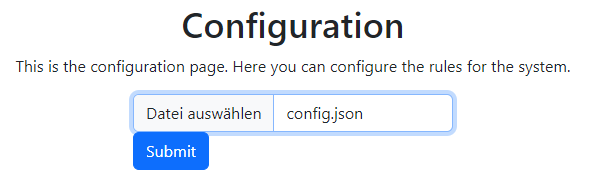
\includegraphics[width=\textwidth]{images/Konfiguration.png}
	\caption[Konfigurationswerkzeug des Prototyps]{
		Screenshot des Konfigurationswerkzeugs des Prototyps.
	}
	\label{pic:konfiguration}
\end{figure}

Das Konfigurationswerkzeug ist ein zentrales Element der Nutzerschnittstelle, um das System zu konfigurieren.
Das Konfigurationswerkzeug des Prototyps ist in \cref{pic:konfiguration} abgebildet, wo zu sehen ist, dass das Konfigurationswerkzeug aus einem Dateiwähler besteht, der es ermöglicht, die Konfiguration im JSON Definitionsformat vom Dateisystem zu laden.
Die geladene Konfiguration wird anschließend mittels des \emph{Submit} Buttons an den POST Endpunkt \emph{/definitions} des Servers gesendet, um die Konfiguration zu setzen.
Realisiert ist das Konfigurationswerkzeug als einzelne React-Komponente \emph{ConfigurationInput}, die den Dateiwähler und die Logik zum Senden der Konfiguration enthält.

\subsubsection{Entwicklung des Dashboards}

\begin{figure}[!htbp]
	\centering
	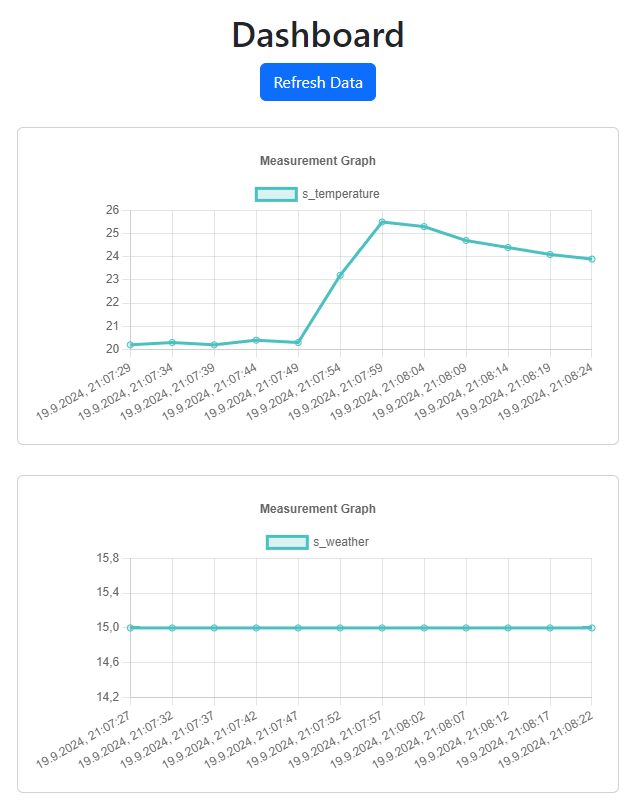
\includegraphics[width=0.95\textwidth]{images/Dashboard.png}
	\caption[Dashboard des Prototyps]{
		Screenshot des Dashboards des Prototyps.
		Abgebildet sind die Diagramme für die Messwerte Temperatur und Regenwahrscheinlichkeit.
	}
	\label{pic:dashboard}
\end{figure}

Das Dashboard ist ein weiteres zentrales Element der Nutzerschnittstelle, um die Messwerte des Systems anzuzeigen.
Es ist in \cref{pic:dashboard} abgebildet, wo zu sehen ist, dass das Dashboard aus Diagrammen besteht, die die Messwerte der Sensoren anzeigen.
Für den Prototyp werden die unterschiedlichen Messwerte jeweils in einem eigenen Diagramm angezeigt, welches mithilfe der \emph{Chart.js}\footnote{\href{https://www.chartjs.org/}{Chart.js}} Bibliothek erstellt wird.
Hierbei werden zwei unterschiedliche React Komponenten verwendet, um das Dashboard zu realisieren.
Die \emph{SingleGraph} Komponente bekommt die Daten für ein einzelnes Diagramm übergeben und ist dafür zuständig, dieses Diagramm mittels \emph{Chart.js} zu erstellen.
Dabei wird die x-Achse als Zeitachse mit den jeweiligen Zeitstempeln und die y-Achse als Messwertachse definiert.
Dies ist im Beispiel ersichtlich, wo der erste Graph die Temperatur in Celsius auf der y-Achse anzeigt und die Zeit als Datums- und Uhrzeitangabe auf der x-Achse.
Dabei wird jede Messung als einzelner Punkt im Diagramm dargestellt, welche durch Linien verbunden sind.
Die Konfiguration, die dieses Beispiel erzeugt hat, ist auf ein Intervall von fünf Sekunden für beide Sensoren eingestellt.
In diesem Beispiel ist auch der zweite Graph zu sehen, der die Wahrscheinlichkeit für Niederschlag in Prozent auf der y-Achse anzeigt.

Die \emph{AllGraphs} Komponente hat einen Button, welcher die Daten für alle Sensoren mittels GET an den Endpunkt \emph{/measurements} des Servers abruft und für jeden Sensor ein \emph{SingleGraph} Diagramm erstellt.
Außerdem ist die Webseite so entwickelt, dass sich die Diagramme automatisch an die Größe des Bildschirms anpassen, sodass sie auch auf mobilen Geräten lesbar sind.

\subsubsection{Zusammenfassung der Entwicklung der Nutzerschnittstelle}
Zusammengefasst besteht die Nutzerschnittstelle aus dem Konfigurationswerkzeug und dem Dashboard, die beide in React implementiert sind.
Das Konfigurationswerkzeug ermöglicht das Laden und Setzen der Konfiguration im JSON-Definitionsformat.
Das Dashboard zeigt die Messwerte des Systems in Diagrammen an, wobei für jeden Sensor ein eigenes Diagramm erstellt wird.


\subsection{Zusammenfassung der Entwicklung des Prototyps}
Zusammengefasst besteht der Prototyp aus mehreren Komponenten sowie einem Definitionsformat, das die Konfiguration des Systems definiert.
Das Definitionsformat ermöglicht es dem Nutzer, Sensoren, Regeln und externe Datenquellen zu definieren.
Diese Regeln können Bedingungen und Aktionen enthalten, wodurch komplexe Abläufe gesteuert werden können.
Die Sensoren können unterschiedliche Typen haben, wie I2C oder Netzwerk, und spezifische Attribute und Aktionen definieren.
Externe Datenquellen können über das Definitionsformat eingebunden werden.

Der Server ist für die Speicherung der Sensordaten, die Verarbeitung von externen Datenquellen und die Verteilung von Benachrichtigungen zuständig.
Außerdem ist er das Bindeglied zwischen dem Sensor- und Aktuatorkoffer und der Nutzerschnittstelle.
Die REST-API des Servers ermöglicht die Kommunikation zwischen den Komponenten.

Der Sensor- und Aktuatorkoffer ist für die Ausführung der durch den Nutzer definierten Regeln und der damit verbundenen Ansteuerung der Sensoren und Aktuatoren zuständig.
Durch laden der Konfiguration kann er die definierten Regeln ausführen und die Sensoren auslesen.

Die Nutzerschnittstelle ist für die Konfiguration des Systems und die Anzeige der Messwerte zuständig.
Das Konfigurationswerkzeug ermöglicht das Laden und Setzen der Konfiguration im JSON-Definitionsformat.
Das Dashboard zeigt die Messwerte des Systems in Diagrammen an.



\section{Zusammenfassung der Implementierung}
Zusammengefasst wurde in diesem Kapitel die Implementierung des Prototyps beschrieben.
Der Prototyp besteht aus einem Hardware- und einem Softwareteil, die jeweils in mehrere Komponenten unterteilt sind.
Der Hardwareteil besteht aus einem Raspberry Pi, der als zentrale Steuereinheit dient, und Sensoren, die an den Raspberry Pi angeschlossen sind.
Der Softwareteil besteht aus dem Server, der die Kommunikation zwischen den Komponenten ermöglicht, dem Sensor- und Aktuatorkoffer, der für die Ausführung der Regeln und die Ansteuerung der Sensoren und Aktuatoren zuständig ist, und der Nutzerschnittstelle, die für die Konfiguration des Systems und die Anzeige der Messwerte zuständig ist.
Die Implementierung des Prototyps erfolgte in Python und JavaScript, wobei für die Kommunikation zwischen den Komponenten eine REST-API verwendet wird.
Im nächsten Kapitel wird der Prototyp evaluiert, wobei ein Fokus auf die Erfüllung der Anforderungen und dem Mehrwert des Systems gegenüber bestehenden Systemen gelegt wird.
